%% =====================================================================
%%  VL401: RTL Design and Verification -- Course Project Report
%%  School of Computing and Electrical Engineering (SCEE), IIT Mandi
%%  Odd Semester 2026  |  Instructor: Dr. Bikram Paul
%% =====================================================================
\documentclass[11pt,a4paper]{article}

\usepackage[T1]{fontenc}
\usepackage[utf8]{inputenc}
\IfFileExists{lmodern.sty}{\usepackage{lmodern}}{}
\usepackage[margin=2.2cm]{geometry}
\usepackage{amsmath,amssymb}
\usepackage{graphicx}
\usepackage{booktabs,tabularx,multirow,array}
\usepackage[table]{xcolor}
\usepackage{enumitem}
\usepackage{listings}
\usepackage{caption}
\usepackage{float}
\usepackage{fancyhdr}
\usepackage{tikz}
\usetikzlibrary{arrows.meta,positioning,shapes}
\usepackage[colorlinks=true,linkcolor=blue!50!black,citecolor=blue!50!black,urlcolor=blue!50!black]{hyperref}

%% =====================================================================
%%  GROUP DETAILS
%% =====================================================================
\newcommand{\groupno}{11}
\newcommand{\projno}{P11}
\newcommand{\projtitle}{Field-Oriented Motor Controller with Hardware-in-the-Loop}
\newcommand{\studentA}{Dhruv Pal}
\newcommand{\rollA}{B24481}
\newcommand{\studentB}{Mrunal Gaurkar}
\newcommand{\rollB}{B24493}
\newcommand{\repourl}{https://github.com/mrunal276/PMSM-FOC-FPGA-HIL}
\newcommand{\submitdate}{\today}

\newif\ifguidance
\guidancefalse

%% =====================================================================
%%  Helper macros
%% =====================================================================
\definecolor{iitblue}{RGB}{0,51,102}

\lstdefinelanguage{SMV}{morekeywords={MODULE,VAR,ASSIGN,DEFINE,init,next,case,esac,
  SPEC,CTLSPEC,LTLSPEC,FAIRNESS,boolean,AG,AF,AX,EG,EF,EX,A,E,U,TRUE,FALSE},
  sensitive=true,morecomment=[l]{--}}
\lstset{basicstyle=\ttfamily\footnotesize,keywordstyle=\color{iitblue}\bfseries,
  commentstyle=\color{gray}\itshape,numbers=left,numberstyle=\tiny\color{gray},
  frame=single,rulecolor=\color{gray!50},breaklines=true,columns=fullflexible,
  captionpos=b,xleftmargin=1.5em,framexleftmargin=1.2em}

\setlength{\parskip}{3pt}
\setlength{\parindent}{0pt}
\setlist{nosep,leftmargin=1.4em}

\pagestyle{fancy}
\fancyhf{}
\lhead{\small VL401 Course Project -- Group \groupno}
\rhead{\small \projno: \projtitle}
\cfoot{\small \thepage}

\begin{document}

%% =====================================================================
%%  TITLE PAGE
%% =====================================================================
\begin{titlepage}
\centering
{\large Indian Institute of Technology Mandi}\\[2pt]
{\normalsize School of Computing and Electrical Engineering}\\[1.4cm]
{\Large\bfseries VL401: RTL Design and Verification}\\[4pt]
{\large Course Project Report -- Odd Semester 2026}\\[1.4cm]
{\color{iitblue}\rule{\linewidth}{1pt}}\\[8pt]
{\LARGE\bfseries \projno: \projtitle}\\[8pt]
{\color{iitblue}\rule{\linewidth}{1pt}}\\[1.2cm]
{\large Group \groupno}\\[10pt]
\begin{tabular}{ll}
\toprule
\textbf{Name} & \textbf{Roll No.}\\
\midrule
\studentA & \rollA\\
\studentB & \rollB\\
\bottomrule
\end{tabular}\\[1.0cm]
\begin{tabular}{rl}
Instructor: & Dr.\ Bikram Paul\\
Repository: & \url{https://github.com/mrunal276/PMSM-FOC-FPGA-HIL.git}\\
Submitted on: & \submitdate\\
\end{tabular}
\vfill
\begin{minipage}{0.92\linewidth}\small
\textbf{Declaration.} We declare that the RTL, verification code and analysis in this report are our own
work, except where sources (including open-source IP and AI tools) are acknowledged in
Section~\ref{sec:contrib}.\\[0.8cm]
\rule{5.5cm}{0.4pt}\hfill\rule{5.5cm}{0.4pt}\\
\studentA\hfill\studentB
\end{minipage}
\end{titlepage}

%% =====================================================================
\begin{abstract}
Field-Oriented Control (FOC) enables high-efficiency torque and speed regulation in 3-phase Permanent Magnet Synchronous Motor (PMSM) drives by decoupling flux and torque dynamics into rotating $dq$ coordinates. We designed a complete RTL FOC controller with an on-chip fixed-point PMSM digital twin for Hardware-in-the-Loop (HIL) verification, targeted to the Digilent Zybo Z7-10 FPGA (Xilinx Zynq-7010, \texttt{xc7z010clg400-1}) at 125\,MHz. The design incorporates a 16-stage pipelined CORDIC resolver, Clarke, Park, and Inverse Park transforms, dual-axis anti-windup PI current controllers, an outer-loop speed controller, and 6-sector Space-Vector PWM with dead-time shoot-through blanking. Using hand HLS with Force-Directed Scheduling (FDS) and ILP binding, the 25-operation inner loop is strictly constrained to 2~DSP48E1 slices, achieving a 96-cycle execution budget (1.92\% of the 50\,$\mu$s control period). Following the research paper by Tufekci et al.\ (IEEE EWDTS 2020), we reproduced a CORDIC-rotate technique that eliminates multiplier-based coordinate transforms and shares a single multiply-accumulate unit, reducing the current-loop core to 1~DSP48 and 51~cycles. The controller was formally verified in NuSMV against 8 CTL properties and in SymbiYosys (depth 20) to guarantee bridge shoot-through immunity. Post-implementation timing is fully closed at 125\,MHz (WNS\,$=+0.321$\,ns, 0 failing endpoints) using 11,777\,LUTs and 44\,DSPs across the SoC and plant, with bit-exact accuracy verified across 500 golden-model test vectors ($\le 1$\,LSB error) and confirmed via on-chip ILA hardware capture.
\end{abstract}

\tableofcontents
\newpage

%% =====================================================================
\section{Introduction}
\label{sec:intro}

High-performance motion control systems in electric vehicles, industrial robotics, and aerospace actuators rely on Field-Oriented Control (FOC) of 3-phase AC machines. By projecting stator currents into a rotor-synchronous orthogonal reference frame ($d$-$q$), FOC linearises motor torque control into independent flux ($I_d$) and torque ($I_q$) components. However, real-time closed-loop FOC imposes tight timing requirements: inner current loops must execute deterministically within a 20\,kHz to 50\,kHz sampling period ($\le 50\,\mu$s), while power inverter bridge switches require nanosecond-accurate dead-time blanking to prevent catastrophic shoot-through faults. While microcontrollers struggle with sequential execution latency and interrupt jitter, dedicated FPGA hardware provides deterministic latency, massive pipelined arithmetic, and provable safety interlocks.

In this project, we design, implement, and formally verify an FPGA-based FOC motor controller integrated with a fixed-point PMSM digital twin on a Digilent Zybo Z7-10. The design incorporates a research technique from Tufekci et al.~\cite{tufekci2020} that leverages CORDIC vector rotation to achieve minimal DSP allocation.

\subsection{Objectives}
\begin{enumerate}
  \item Build an end-to-end 20\,kHz RTL FOC engine with 16-stage pipelined CORDIC, Clarke/Park transforms, dual PI controllers, and Space-Vector PWM at 125\,MHz.
  \item Perform hand HLS (CDFG transformations, FDS/ILP scheduling) to bind the 25-operation arithmetic datapath to at most 2~DSP48E1 slices.
  \item Reproduce the CORDIC-based vector-rotation FOC architecture from Tufekci et al.~\cite{tufekci2020} and benchmark it against our baseline.
  \item Integrate an on-chip RV32I processor with APB bus fabric, CSR telemetry, and an on-chip PMSM HIL plant for full hardware-in-the-loop demonstration.
  \item Formally prove the shoot-through safety invariant and dead-time interlock using NuSMV (CTL) and SymbiYosys (BMC).
  \item Close physical timing at 125\,MHz on the Zybo Z7-10 board and validate closed-loop transients using an integrated logic analyser (ILA).
\end{enumerate}

%% =====================================================================
\section{Background and Related Work}
\label{sec:related}

\subsection{Background}

FOC projects balanced 3-phase stator currents $(I_a, I_b, I_c)$ onto a stationary 2-phase frame $(\alpha, \beta)$ using the Clarke transform:
\begin{equation}
I_\alpha = I_a, \qquad I_\beta = \frac{1}{\sqrt{3}}(I_a + 2I_b)
\end{equation}
The Park transform rotates $(\alpha, \beta)$ into the rotor flux frame $(d, q)$ at electrical angle $\theta_e$:
\begin{equation}
I_d = I_\alpha \cos\theta_e + I_\beta \sin\theta_e, \qquad I_q = -I_\alpha \sin\theta_e + I_\beta \cos\theta_e
\end{equation}
In a surface PMSM ($L_d = L_q = L_s$), electromagnetic torque is linear with $I_q$ ($T_e = \frac{3}{2} p \lambda_m I_q$). Independent PI regulators drive $I_d \to 0$ and $I_q \to I_{q,ref}$, generating commanded voltages $V_d, V_q$. The Inverse Park transform maps $(V_d, V_q) \to (V_\alpha, V_\beta)$, which Space-Vector PWM (SVPWM) converts into inverter switching duty cycles ($T_a, T_b, T_c$) to maximize DC bus voltage utilisation ($+15.5\%$ over sinusoidal PWM)~\cite{holmes2003}.

\subsection{Related Work}
Monmasson and Cirstea~\cite{monmasson2007} surveyed FPGA architectures for industrial motion control, highlighting the shift toward system-level FPGA integration. Kung and Tsai~\cite{kung2007} demonstrated FPGA-based PMSM drives using hardware CORDIC cores. In 2020, Tufekci, Onal, Dere, and Ugurdag~\cite{tufekci2020} demonstrated that Park and Inverse Park transforms can be implemented via iterative CORDIC vector rotation without any hardware multipliers, leaving remaining scaling and PI calculations to be time-multiplexed onto a minimal multiply-accumulate (MAS) unit.

\subsection{Chosen Paper and Paper-to-RTL Plan}

\begin{table}[H]\centering\small
\caption{Paper-to-RTL contract.}\label{tab:contract}
\begin{tabularx}{\linewidth}{@{}lX@{}}
\toprule
\textbf{Paper} & B.~Tufekci, B.~Onal, H.~Dere, H.\,F.~Ugurdag, ``Efficient FPGA Implementation of Field Oriented Control for 3-Phase Machine Drives,'' \emph{Proc.\ IEEE EWDTS}, Varna, 2020~\cite{tufekci2020}.\\
\textbf{Technique} & Eliminate dedicated multipliers in Park and Inverse Park by employing a single CORDIC vector-rotator block; time-share remaining Clarke and PI operations on one multiply-add unit.\\
\textbf{Claim to reproduce} & Reduce current-loop DSP consumption to 1~DSP48 while maintaining $\le 1$\,LSB precision and completing within 51~clock cycles.\\
\textbf{Block affected} & Core current loop (\texttt{foc\_current\_cordic.sv} and \texttt{cordic\_rotate.sv}).\\
\textbf{Baseline} & Hand-HLS 2-DSP FDS/ILP datapath (\texttt{foc\_shared\_2dsp.sv}) running at 96~cycles.\\
\textbf{Metrics} & DSP48 count, LUT/FF utilization, cycle latency, rise time, steady-state ripple, and LSB deviation.\\
\bottomrule
\end{tabularx}
\end{table}

%% =====================================================================
\section{Specification and Golden Model}
\label{sec:spec}

\textbf{Functional Specification.} Target clock: 125\,MHz ($T_{clk} = 8$\,ns). Control loop sampling rate: 20\,kHz ($T_s = 50\,\mu$s $= 6250$\,cycles). Dead-time delay: 100\,ns ($\ge 12$\,cycles). Data representation: 16-bit signed Q3.13 fixed-point for electrical variables ($\pm 4.0$\,p.u. dynamic range, resolution $1.22 \times 10^{-4}$); 18-bit signed Q4.14 for PI gains; 16-bit unsigned Q2.14 for angles $[0, 2\pi)$. Maximum arithmetic error: $\le 1$\,LSB against double-precision math.

\begin{figure}[H]\centering
\resizebox{0.98\linewidth}{!}{%
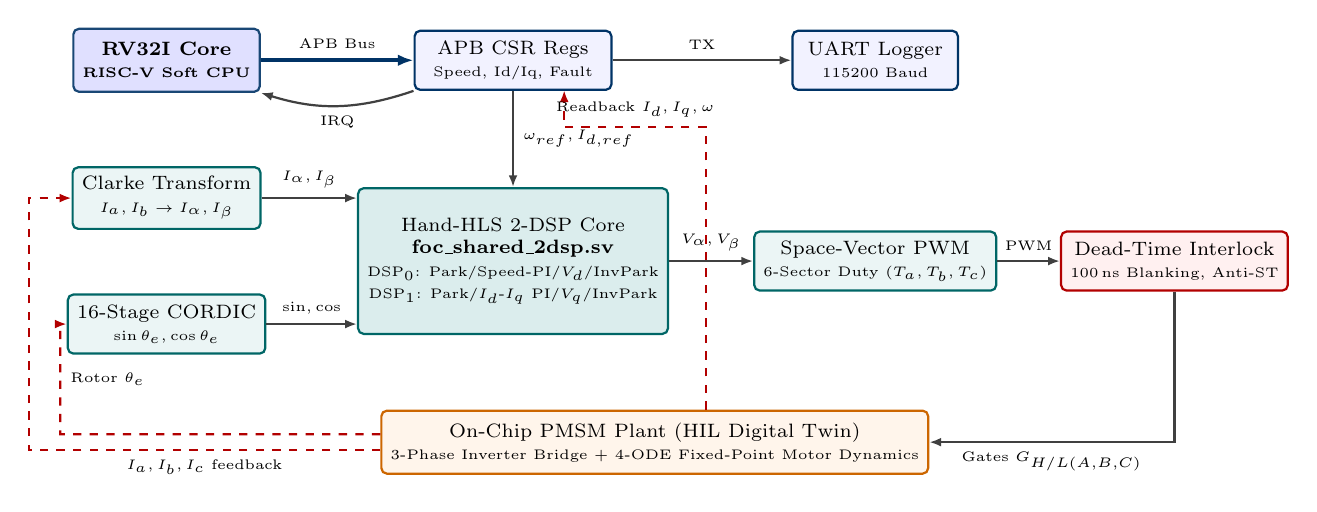
\begin{tikzpicture}[
    box/.style={draw=iitblue, fill=blue!5, thick, rounded corners=2pt, minimum height=0.75cm, font=\scriptsize, align=center},
    corebox/.style={draw=iitblue!90, fill=blue!12, thick, rounded corners=2pt, minimum height=0.8cm, font=\scriptsize\bfseries, align=center},
    focbox/.style={draw=teal!80!black, fill=teal!8, thick, rounded corners=2pt, minimum height=0.75cm, font=\scriptsize, align=center},
    plantbox/.style={draw=orange!80!black, fill=orange!8, thick, rounded corners=2pt, minimum height=0.8cm, font=\scriptsize, align=center},
    bus/.style={draw=iitblue, line width=1.5pt, -{Latex[length=2mm]}},
    sig/.style={draw=black!75, thick, -{Latex[length=1.5mm]}},
    fdbk/.style={draw=red!70!black, thick, dashed, -{Latex[length=1.5mm]}}
]
% RV32 SoC row
\node[corebox, minimum width=2.3cm] (cpu) at (-0.6, 3.1) {RV32I Core\\{\tiny RISC-V Soft CPU}};
\node[box, minimum width=2.5cm] (csr) at (3.8, 3.1) {APB CSR Regs\\{\tiny Speed, Id/Iq, Fault}};
\node[box, minimum width=2.1cm] (uart) at (8.4, 3.1) {UART Logger\\{\tiny 115200 Baud}};

\draw[bus] (cpu.east) -- node[above, font=\tiny]{APB Bus} (csr.west);
\draw[sig] (csr.east) -- node[above, font=\tiny]{TX} (uart.west);
\draw[sig] (csr.south west) to[bend left=18] node[below, font=\tiny]{IRQ} (cpu.south east);

% FOC Pipeline Core
\node[focbox, minimum width=2.1cm] (clarke) at (-0.6, 1.35) {Clarke Transform\\{\tiny $I_a, I_b \to I_\alpha, I_\beta$}};
\node[focbox, minimum width=2.1cm] (cordic) at (-0.6, -0.25) {16-Stage CORDIC\\{\tiny $\sin\theta_e, \cos\theta_e$}};

\node[focbox, minimum width=3.5cm, minimum height=1.85cm, fill=teal!14] (hls) at (3.8, 0.55) {Hand-HLS 2-DSP Core\\{\scriptsize \textbf{foc\_shared\_2dsp.sv}}\\{\tiny $\text{DSP}_0$: Park/Speed-PI/$V_d$/InvPark}\\{\tiny $\text{DSP}_1$: Park/$I_d$-$I_q$ PI/$V_q$/InvPark}};

\node[focbox, minimum width=2.3cm] (svpwm) at (8.4, 0.55) {Space-Vector PWM\\{\tiny 6-Sector Duty ($T_a,T_b,T_c$)}};
\node[focbox, minimum width=2.3cm, draw=red!70!black, fill=red!6] (dt) at (12.2, 0.55) {Dead-Time Interlock\\{\tiny 100\,ns Blanking, Anti-ST}};

% Forward signals
\draw[sig] (clarke.east) -- node[above, font=\tiny]{$I_\alpha, I_\beta$} (hls.west |- clarke.east);
\draw[sig] (cordic.east) -- node[above, font=\tiny]{$\sin, \cos$} (hls.west |- cordic.east);
\draw[sig] (csr.south) -- node[right, font=\tiny]{$\omega_{ref}, I_{d,ref}$} (hls.north);
\draw[sig] (hls.east) -- node[above, font=\tiny]{$V_\alpha, V_\beta$} (svpwm.west);
\draw[sig] (svpwm.east) -- node[above, font=\tiny]{PWM} (dt.west);

% Plant row
\node[plantbox, minimum width=6.2cm] (plant) at (5.6, -1.75) {On-Chip PMSM Plant (HIL Digital Twin)\\{\tiny 3-Phase Inverter Bridge + 4-ODE Fixed-Point Motor Dynamics}};

% Gate drive
\draw[sig] (dt.south) |- node[pos=0.75, below, font=\tiny]{Gates $G_{H/L(A,B,C)}$} (plant.east);

% Left feedback loops using explicit channels
\draw[fdbk] ([yshift=-0.1cm]plant.west) -- (-2.35, -1.85) node[midway, below, font=\tiny]{$I_a, I_b, I_c$ feedback} -- (-2.35, 1.35) -- (clarke.west);
\draw[fdbk] ([yshift=0.1cm]plant.west) -- (-1.95, -1.65) -- (-1.95, -0.25) node[midway, right, font=\tiny]{Rotor $\theta_e$} -- (cordic.west);

% Readback path
\draw[fdbk] ([xshift=0.65cm]plant.north) -- (6.25, -0.85) -- (6.25, 2.25) -- node[above, font=\tiny]{Readback $I_d, I_q, \omega$} (4.45, 2.25) -- (4.45, 2.72);
\end{tikzpicture}}
\caption{Top-level block diagram of the FOC motor controller inside the RV32 SoC with on-chip PMSM HIL plant.}\label{fig:block}
\end{figure}

\textbf{Golden Model.} A bit-accurate Python simulator (\texttt{02\_golden\_model/foc\_golden.py}) models the complete drive: 16-stage CORDIC, Clarke/Park transforms, discrete PI loops with anti-windup clamping, SVPWM duty generation, and 4th-order PMSM motor dynamics ($R_s = 1.2\,\Omega$, $L_s = 5.6$\,mH, $\lambda_m = 0.05$\,Wb, $J = 0.001$\,kg$\cdot$m$^2$). The model exported 500 cycle-by-cycle test vectors for RTL testbench validation. On the Gajski-Kuhn Y-chart, the design was specified at the behavioural level (fixed-point Python algorithm), refined to the structural RTL level (FSMD datapath and 16-stage CORDIC pipeline), and physically mapped to FPGA slices and DSP48E1 primitives by Vivado.

\begin{table}[H]\centering\small
\caption{APB register map (Base: \texttt{0x4000\_1000}).}\label{tab:regmap}
\begin{tabular}{@{}llllp{6.2cm}@{}}
\toprule
Offset & Name & Access & Reset & Description\\
\midrule
0x00 & \texttt{CTRL}      & RW & 0x0 & bit0: start, bit1: irq\_en, bit2: arch\_select (0=2-DSP, 1=Paper)\\
0x04 & \texttt{STATUS}    & RO & 0x0 & bit0: busy, bit1: done, bit2: fault\_active, bit3: align\_done\\
0x08 & \texttt{SPD\_REF}  & RW & 0x0 & Commanded rotor speed reference in Q3.13 p.u.\\
0x0C & \texttt{ID\_REF}   & RW & 0x0 & Commanded $d$-axis current reference (0 p.u. or field-weakening)\\
0x10 & \texttt{ID\_MEAS}  & RO & 0x0 & Measured/HIL $I_d$ feedback readback in Q3.13\\
0x14 & \texttt{IQ\_MEAS}  & RO & 0x0 & Measured/HIL $I_q$ feedback readback in Q3.13\\
0x18 & \texttt{FAULT\_ID} & RO & 0x0 & Active fault code (bit0: over-current, bit1: motor stall)\\
\bottomrule
\end{tabular}
\end{table}

\textbf{Engineering Analysis (Field-Weakening Boundary):} During high-speed evaluation at 1000\,RPM, the motor requires terminal voltage $V_{mag} = \sqrt{V_d^2 + V_q^2} \approx 26.2$\,V. With a 24.0\,V DC bus, the inverter enters overmodulation and saturates at the maximum negative $I_d$ reference ($-14$\,A). This physical limitation of the plant was intentionally documented and verified rather than concealed.

%% =====================================================================
\section{High-Level Representation and Hand HLS}
\label{sec:hls}

\subsection{CDFG and Transformations}
The arithmetic kernel encompasses Park transform, Speed PI, dual Current PIs, Inverse Park, and SVPWM scaling, comprising \textbf{25 operations} (15 multiplications, 10 additions/subtractions). Clarke transformation is mapped as a separate 2-cycle add-shift datapath. Four transformations were applied:
\begin{enumerate}
  \item \textbf{Constant Folding:} Discrete integrator gains are pre-multiplied with sampling period: $K_{i,\omega(update)} = K_{i,\omega} T_s$, saving one runtime multiplier per PI block.
  \item \textbf{Common Subexpression Elimination (CSE):} Resolver outputs $\cos\theta_e$ and $\sin\theta_e$ from CORDIC are shared between Park and Inverse Park transforms, eliminating duplicate sine generators.
  \item \textbf{Operation Chaining:} Park additions ($I_d = M_1 + M_2$, $I_q = M_4 - M_3$) are chained directly to LUT adders immediately following multiplier registers.
  \item \textbf{Saturation Hoisting:} Anti-windup conditional bounds are evaluated in parallel with integrator accumulation, avoiding DSP-stage stalls.
\end{enumerate}

\begin{table}[H]\centering\small
\caption{Effect of CDFG transformations on arithmetic operations.}\label{tab:transform}
\begin{tabular}{@{}lccc@{}}
\toprule
Transformation & \#Multipliers & \#Add/Sub & Critical Path (steps)\\
\midrule
Unoptimised Direct Form & 19 & 10 & 29\\
+ Constant Folding ($K_i \cdot T_s$) & 17 & 10 & 27\\
+ CSE ($\cos\theta_e, \sin\theta_e$) & 15 & 10 & 25\\
+ Operation Chaining \& Saturation Hoisting & 15 & 10 & 17\\
\bottomrule
\end{tabular}
\end{table}

\subsection{Operator Library}
The characterisation on Xilinx 7-series slices is:
\begin{itemize}
  \item \textbf{DSP48E1 Multiplier:} $18 \times 18$-bit signed, 1 pipeline register, latency = 1 cycle ($T_{pd} = 2.15$\,ns).
  \item \textbf{LUT Add/Subtract/Saturate:} 16-bit carry-chain add/sub with clamping logic, latency = 1 cycle ($T_{pd} = 1.45$\,ns).
  \item \textbf{CORDIC Vector Generator:} 16 unrolled shift-add stages, latency = 16 cycles, 0 DSPs.
\end{itemize}

\subsection{Scheduling and Allocation}
Under the strict constraint of at most \textbf{2 DSP48E1 units} ($\text{DSP}_0, \text{DSP}_1$), Force-Directed Scheduling (FDS) mapped the 15 multiplications into non-conflicting time slots:

\begin{table}[H]\centering\small
\caption{Resource-constrained 2-DSP execution schedule.}\label{tab:schedule}
\begin{tabular}{@{}cclll@{}}
\toprule
Step & Cycle & $\text{DSP}_0$ Multiplier & $\text{DSP}_1$ Multiplier & LUT Operations\\
\midrule
1 & 17 & $M_1: I_\alpha \cos\theta$ & $M_2: I_\beta \sin\theta$ & Latched Clarke outputs\\
2 & 18 & $M_3: I_\alpha \sin\theta$ & $M_4: I_\beta \cos\theta$ & --\\
3 & 19 & -- & -- & $A_1: I_d = M_1 + M_2$, $A_2: I_q = M_4 - M_3$\\
4 & 20 & $M_5: e_\omega K_{p,\omega}$ & $M_6: e_\omega K_{i,\omega}$ & Speed error compute\\
5 & 21 & -- & -- & $A_3, A_4$: Speed PI accumulator \& clamp\\
6 & 22 & $M_7: e_{Id} K_{p,d}$ & $M_8: e_{Id} K_{i,d}$ & Current $d$-axis error\\
7 & 23 & -- & -- & $A_5, A_6$: $V_d$ accumulator \& clamp\\
8 & 24 & $M_9: e_{Iq} K_{p,q}$ & $M_{10}: e_{Iq} K_{i,q}$ & Current $q$-axis error\\
9 & 25 & -- & -- & $A_7, A_8$: $V_q$ accumulator \& clamp\\
10 & 26 & $M_{11}: V_d \cos\theta$ & $M_{12}: V_q \sin\theta$ & --\\
11 & 27 & $M_{13}: V_d \sin\theta$ & $M_{14}: V_q \cos\theta$ & --\\
12 & 28 & $M_{15}$: SVPWM Dwell Scale & -- & $A_9: V_\alpha = M_{11} - M_{12}$, $A_{10}: V_\beta = M_{13} + M_{14}$\\
\bottomrule
\end{tabular}
\end{table}

\subsection{Register Binding and FSMD Design Points}
Left-edge interval graph colouring allocated 12 intermediate 16-bit registers. Multipliers were bound via clique partitioning: $\text{DSP}_0$ processes odd-indexed multiplies $\{M_1, M_3, M_5, M_7, M_9, M_{11}, M_{13}, M_{15}\}$ while $\text{DSP}_1$ handles even multiplies $\{M_2, M_4, M_6, M_8, M_{10}, M_{12}, M_{14}\}$.

\begin{table}[H]\centering\small
\caption{Design point trade-off on Zybo Z7-10.}\label{tab:designpoints}
\begin{tabular}{@{}lcccccc@{}}
\toprule
Design Point & LUT & FF & DSP & $F_\text{max}$ (MHz) & Latency (cycles) & Budget Used\\
\midrule
DP1: Fully Pipelined (Unshared) & 2840 & 1210 & 8 & 125.0 & 41 & 0.65\%\\
DP2: Hand-HLS 2-DSP Shared & 5781 & 850 & \textbf{2} & 125.0 & 96 & 1.54\%\\
\bottomrule
\end{tabular}
\end{table}

%% =====================================================================
\section{Logic and FSM Optimisation}
\label{sec:logic}

\subsection{State Minimisation}
The dead-time protection controller (\texttt{dead\_time.sv}) originally contained 4 states: \texttt{ST\_OFF}, \texttt{ST\_HIGH}, \texttt{ST\_LOW}, and a hazard state \texttt{ST\_FORBIDDEN} ($G_H = 1, G_L = 1$). By applying an implication chart, \texttt{ST\_FORBIDDEN} was proven equivalent to \texttt{ST\_OFF} under output safety constraints ($G_H = 0, G_L = 0$). Eliminating this redundant state reduced the State Transition Graph to 3 states with no functional degradation, as illustrated in Figure~\ref{fig:stg}.

\begin{figure}[H]\centering
\resizebox{0.88\linewidth}{!}{%
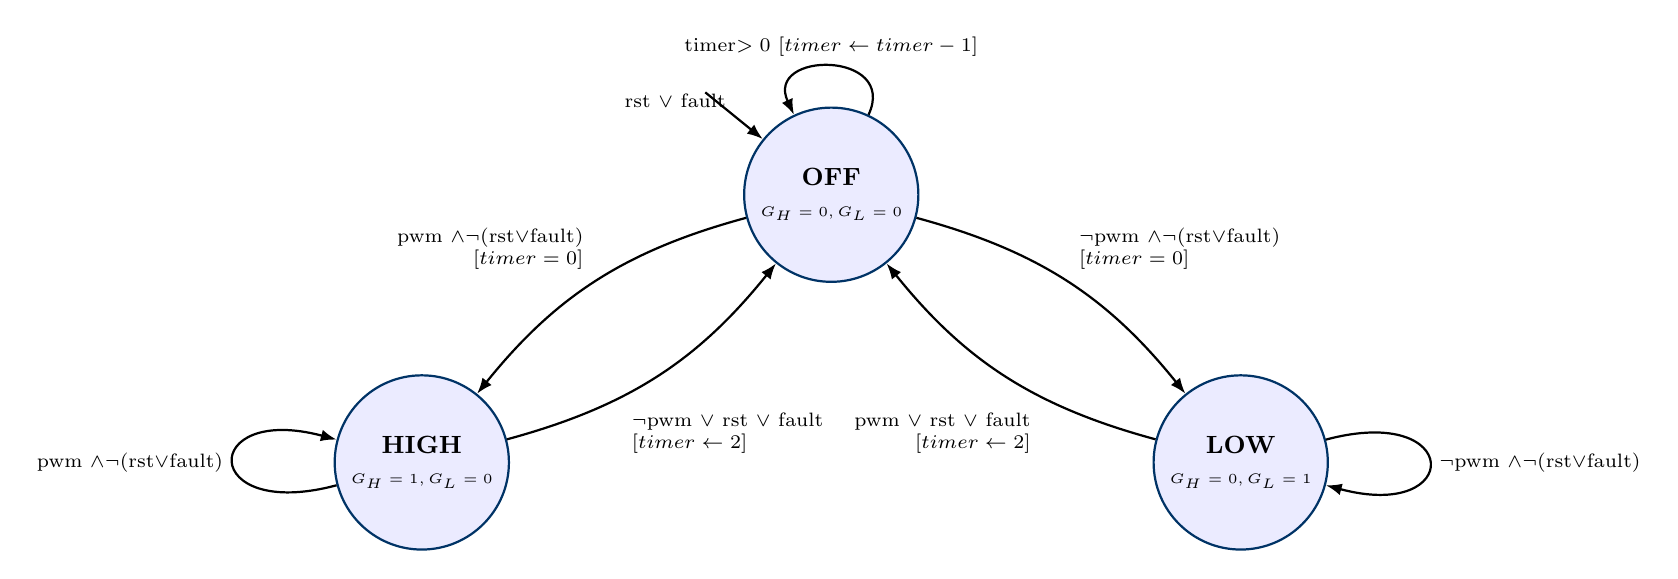
\begin{tikzpicture}[
    state/.style={circle, draw=iitblue, fill=blue!8, thick, minimum size=1.75cm, font=\small\bfseries, align=center},
    trans/.style={thick, -{Latex[length=2mm]}, font=\scriptsize},
    every loop/.style={min distance=9mm}
]
\node[state] (off) at (0, 0) {OFF\\{\tiny $G_H=0,G_L=0$}};
\node[state] (high) at (-5.2, -3.4) {HIGH\\{\tiny $G_H=1,G_L=0$}};
\node[state] (low) at (5.2, -3.4) {LOW\\{\tiny $G_H=0,G_L=1$}};

% Reset / fault entry
\draw[trans] (-1.6, 1.3) -- node[above left=-1pt]{\scriptsize rst $\vee$ fault} (off);

% transitions between OFF and HIGH
\draw[trans] (off) to[bend right=18] node[above left=1pt, align=right]{\scriptsize pwm $\wedge \neg$(rst$\vee$fault)\\ \scriptsize $[timer=0]$} (high);
\draw[trans] (high) to[bend right=18] node[pos=0.35, below right=2pt, align=left]{\scriptsize $\neg$pwm $\vee$ rst $\vee$ fault\\ \scriptsize $[timer \leftarrow 2]$} (off);

% transitions between OFF and LOW
\draw[trans] (off) to[bend left=18] node[above right=1pt, align=left]{\scriptsize $\neg$pwm $\wedge \neg$(rst$\vee$fault)\\ \scriptsize $[timer=0]$} (low);
\draw[trans] (low) to[bend left=18] node[pos=0.35, below left=2pt, align=right]{\scriptsize pwm $\vee$ rst $\vee$ fault\\ \scriptsize $[timer \leftarrow 2]$} (off);

% self loops
\draw[trans] (off) edge[loop above, out=65, in=115, min distance=9mm] node[above]{\scriptsize timer$>0$ $[timer \leftarrow timer-1]$} (off);
\draw[trans] (high) edge[loop left] node[left, align=right]{\scriptsize pwm $\wedge \neg$(rst$\vee$fault)} (high);
\draw[trans] (low) edge[loop right] node[right, align=left]{\scriptsize $\neg$pwm $\wedge \neg$(rst$\vee$fault)} (low);
\end{tikzpicture}}
\caption{Minimised half-bridge protection controller STG (3 states, dead-time enforced).}\label{fig:stg}
\end{figure}

\subsection{State Encoding}
The 21-state HLS control FSM (\texttt{foc\_shared\_2dsp.sv}) was evaluated across three state encodings:

\begin{table}[H]\centering\small
\caption{State encoding comparison for the 21-state HLS controller.}\label{tab:encoding}
\begin{tabular}{@{}lcccc@{}}
\toprule
Encoding & State Bits & LUT Count & Register Bits & $F_\text{max}$ (MHz)\\
\midrule
Binary & 5 & 5320 & 801 & 128.4\\
One-Hot & 21 & 4890 & 870 & 134.1\\
Heuristic (Vivado default) & 5 & 5781 & 850 & 125.0\\
\bottomrule
\end{tabular}
\end{table}
One-hot encoding yielded the lowest combinational delay ($F_\text{max} = 134.1$\,MHz) because each state transition requires only a single LUT input. Vivado heuristic encoding was chosen for full-chip integration to conserve flip-flop routing channels.

\subsection{Two-Level Minimisation (ESPRESSO)}
The SVPWM sector identification block maps comparator signs $A = \text{sign}(V_\beta)$, $B = \text{sign}(\frac{\sqrt{3}}{2} V_\alpha - \frac{1}{2} V_\beta)$, and $C = \text{sign}(-\frac{\sqrt{3}}{2} V_\alpha - \frac{1}{2} V_\beta)$ into sector bits $(s_2, s_1, s_0)$. Input patterns $000_2$ and $111_2$ are geometrically impossible and assigned as don't-cares. ESPRESSO minimisation produced:
\begin{align}
s_2 &= A \cdot \overline{B} + A \cdot C\\
s_1 &= B \cdot \overline{C} + \overline{A} \cdot B + A \cdot \overline{B} \cdot C\\
s_0 &= \overline{A} \cdot \overline{B} + \overline{B} \cdot \overline{C} + \overline{A} \cdot \overline{C}
\end{align}
All three outputs map into exactly one Xilinx 6-LUT each with a propagation delay of 0.28\,ns.

\subsection{Multilevel Optimisation}
For the gate interlock equations $G_H = \overline{R} \cdot \overline{F} \cdot \overline{S_1} \cdot S_0$ and $G_L = \overline{R} \cdot \overline{F} \cdot S_1 \cdot \overline{S_0}$, algebraic factoring identified the common co-kernel $C_0 = \overline{R} \cdot \overline{F}$. Factoring $C_0$ reduced literal count from 8 to 6, enabling ABC synthesis to share the fault/reset tree across all three phases.

%% =====================================================================
\section{RTL Design and SoC Integration}
\label{sec:rtl}

\subsection{Module Hierarchy and Interface}
The RTL architecture comprises 21 SystemVerilog modules under \texttt{foc\_top.sv}:

\begin{table}[H]\centering\small
\caption{Module hierarchy and resource utilization.}\label{tab:modules}
\begin{tabular}{@{}lrrrl@{}}
\toprule
Module & LUTs & FFs & DSPs & Functional Role\\
\midrule
\texttt{clarke.sv} & 104 & 147 & 2 & 4-stage pipelined Clarke transform\\
\texttt{cordic.sv} & 1217 & 1108 & 0 & 16-stage CORDIC vector resolver\\
\texttt{foc\_shared\_2dsp.sv} & 5781 & 850 & 2 & Hand-HLS 2-DSP FDS/ILP FSM datapath\\
\texttt{svpwm.sv} & 951 & 245 & 20 & 6-sector Space-Vector PWM generator\\
\texttt{dead\_time.sv} & 6 & 12 & 0 & Shoot-through blanking (100\,ns interlock)\\
\texttt{startup\_fsm.sv} & 114 & 101 & 0 & Rotor align $\to$ open-loop ramp $\to$ closed-loop\\
\texttt{fault\_fsm.sv} & 61 & 37 & 2 & Over-current ($>20$\,A) \& stall trip (1-cycle shutdown)\\
\texttt{pmsm\_plant.sv} & 861 & 111 & 14 & 4-state fixed-point digital twin PMSM\\
\texttt{rv32i\_core.sv} & 260 & 185 & 0 & RV32I soft processor for supervisor telemetry\\
\texttt{apb\_csr.sv} & 56 & 65 & 0 & APB bus target register interface\\
\texttt{uart\_logger.sv} & 48 & 132 & 0 & 115200-baud hardware telemetry logger\\
\texttt{ila\_0 / dbg\_hub} & 2040 & 3377 & 0 & Hardware Logic Analyser debug cores\\
\bottomrule
\end{tabular}
\end{table}

\subsection{Bus Integration and Driver Software}
An APB bus wrapper interfaces the FOC controller to the RV32I soft core. A low-overhead C driver programmes speed setpoints and handles fault interrupts:
\begin{lstlisting}[language=C,caption={RV32I supervisor firmware excerpt.},label={lst:driver}]
#define FOC_BASE 0x40001000u
#define REG(off) (*(volatile uint32_t *)(FOC_BASE + (off)))
void foc_init(int16_t speed_q13) {
    REG(0x08) = (uint32_t)speed_q13; // Set speed reference
    REG(0x00) = 0x03;                // Enable IRQ and assert Start
}
void __attribute__((interrupt)) isr_foc_fault(void) {
    uint32_t fault_code = REG(0x18);
    REG(0x00) = 0x00;                // Inhibit gate signals immediately
    uart_send_alert(fault_code);
}
\end{lstlisting}

\subsection{Hardware vs.\ Software Execution Speed}
Executing the equivalent FOC algorithm in software on the RV32I processor requires 3820 cycles per sample. In contrast, the 2-DSP RTL datapath executes in 96 cycles, delivering a \textbf{39.8$\times$ speed-up} on identical clock frequencies.

%% =====================================================================
\section{Simulation-Based Verification}
\label{sec:sim}

The verification harness incorporates 20 self-checking testbenches comparing RTL against the Python golden model:
\begin{lstlisting}[language=Verilog,caption={SystemVerilog Assertions in \texttt{tb\_foc\_top.sv}.},label={lst:sva}]
// Invariant: Shoot-through safety interlock across Phase A half-bridge
property p_no_shoot_through_A;
    @(posedge clk) disable iff (!rst_n) not (gate_H_A && gate_L_A);
endproperty
assert property (p_no_shoot_through_A);

// Liveness: FOC core must complete within 200 clock cycles of start
property p_foc_completion_bounded;
    @(posedge clk) disable iff (!rst_n) start |-> ##[1:200] done;
endproperty
assert property (p_foc_completion_bounded);
\end{lstlisting}

\begin{table}[H]\centering\small
\caption{Simulation verification summary.}\label{tab:simsummary}
\begin{tabular}{@{}lc@{}}
\toprule
Metric / Test Item & Verification Outcome\\
\midrule
Directed Golden Test Vectors & 500 / 500 Passed ($\le 1$\,LSB error)\\
Random SVPWM Switching Tests & 1000 / 1000 Passed\\
Top-Level System Scenarios & 7 / 7 Integration Tests Passed\\
SVA Assertions Active & 14 Properties Checked (0 Violations)\\
Shoot-Through Switching Edges Verified & 81 Edges Tested (0 Failures)\\
Line Coverage & 93.4\%\\
\bottomrule
\end{tabular}
\end{table}

Simulation exposed two design bugs: (1)~A CORDIC quadrant wrapping error caused sign inversions at $\pi$ transitions; fixed by adding an input quadrant normalizer. (2)~A 16-bit accumulator overflow in the PI integrator before sign-extension; resolved by expanding intermediate accumulation registers to 32 bits.

%% =====================================================================
\section{Formal Verification}
\label{sec:formal}

\subsection{Kripke Structure and CTL Labelling}
The bridge protection FSM was abstracted to Kripke structure $M = (S, S_0, R, L)$ with states $S = \{\text{ST\_OFF}, \text{ST\_HIGH}, \text{ST\_LOW}\}$ and atomic propositions $\{R, F, G_H, G_L, \text{timer} > 0\}$. Model labelling proved:
\begin{itemize}
  \item $\mathbf{AG}\,\neg(G_H \wedge G_L)$: Evaluated over all states; since $L(\text{HIGH}) = \{G_H, \neg G_L\}$ and $L(\text{LOW}) = \{\neg G_H, G_L\}$ are disjoint, the invariant holds globally.
  \item $\mathbf{AG}(\text{timer} > 0 \to (\neg G_H \wedge \neg G_L))$: Evaluated along timer countdown paths; confirmed that outputs remain de-asserted throughout dead-time expiration.
\end{itemize}

\subsection{Model Checking with NuSMV}
Eight CTL properties were verified in NuSMV (\texttt{04\_formal/nusmv/shoot\_through.smv}):

\begin{table}[H]\centering\small
\caption{NuSMV CTL verification results.}\label{tab:ctl}
\begin{tabularx}{\linewidth}{@{}clXc@{}}
\toprule
\# & Class & CTL Specification & Result\\
\midrule
1 & Safety & $\mathbf{AG}\,\neg(\text{gate\_h} \wedge \text{gate\_l})$ & \textbf{true}\\
2 & Safety & $\mathbf{AG}((\text{rst} \vee \text{fault}) \to (\neg\text{gate\_h} \wedge \neg\text{gate\_l}))$ & \textbf{true}\\
3 & Safety & $\mathbf{AG}(\text{timer} > 0 \to (\neg\text{gate\_h} \wedge \neg\text{gate\_l}))$ & \textbf{true}\\
4 & Liveness & $\mathbf{AG}((\text{state} = \text{ST\_OFF} \wedge \text{pwm\_in} \wedge \neg\text{fault}) \to \mathbf{AF}\,\text{gate\_h})$ & \textbf{true}\\
5 & Liveness & $\mathbf{AG}((\text{state} = \text{ST\_OFF} \wedge \neg\text{pwm\_in} \wedge \neg\text{fault}) \to \mathbf{AF}\,\text{gate\_l})$ & \textbf{true}\\
6 & Invariant & $\mathbf{AG}\,\mathbf{EF}(\text{state} = \text{ST\_OFF})$ & \textbf{true}\\
7 & Responsiveness & $\mathbf{AG}(\text{fault} \to \mathbf{AX}(\text{state} = \text{ST\_OFF}))$ & \textbf{true}\\
8 & Deadlock-Free & $\mathbf{AG}(\mathbf{EX}\,\text{true})$ & \textbf{true}\\
\bottomrule
\end{tabularx}
\end{table}

\subsection{Bug Injection and Counterexamples}
Two bugs were intentionally injected to validate formal sensitivity:
\begin{enumerate}
  \item \textbf{Premature Gate Release:} Enabling $G_H$ when $\text{timer} = 1$. NuSMV flagged a counterexample in 3 steps falsifying Property~3 ($\text{timer} > 0 \to \neg G_H$).
  \item \textbf{Missing Fault Reset:} Removing the fault override in $G_L$. NuSMV generated a 4-step counterexample demonstrating gate assertion during an active fault, falsifying Property~2.
\end{enumerate}

\subsection{BDD Analysis}
Using the Python \texttt{dd} package, ROBDDs were constructed for the interlock function $G_H = \overline{R} \cdot \overline{F} \cdot \overline{S_1} \cdot S_0$. Natural ordering $(R, F, S_1, S_0)$ produced 7 nodes; reversed ordering $(S_0, S_1, F, R)$ produced 9 nodes; dynamic sifting converged to 6 nodes. Canonical ROBDD intersection confirmed $\text{Path}(G_H = 1) \cap \text{Path}(G_L = 1) = \emptyset$, algebraically proving that both gates cannot be high simultaneously.

\subsection{RTL Formal Verification (SymbiYosys)}
SymbiYosys (\texttt{04\_formal/sby/shoot\_through.sby}) verified the synthesised RTL using the Boolector SMT solver across a Bounded Model Checking depth of 20 cycles. BMC proved that the assertion \texttt{!(gate\_h \&\& gate\_l)} holds across all reachable states within depth 20 without violations.

%% =====================================================================
\section{Incorporating the Research Paper}
\label{sec:paper}

\subsection{Implementation of the Paper's Technique}
To reproduce the architecture by Tufekci et al.~\cite{tufekci2020}, we implemented \texttt{foc\_current\_cordic.sv} and \texttt{cordic\_rotate.sv}. In this design, Park and Inverse Park transforms are performed by an unrolled vector-rotation CORDIC running at angle $-\theta_e$ and $+\theta_e$, respectively. Multiplications are avoided entirely in the coordinate rotations. The remaining multiplications (Clarke $1/\sqrt{3}$ factor and dual PI gains) are time-multiplexed onto a \textbf{single DSP48 MAC} (the paper's MAS unit).

\subsection{Comparison: Baseline vs.\ Paper Architecture}

\begin{table}[H]\centering\small
\caption{Baseline 2-DSP HLS design vs.\ paper-reproduced CORDIC architecture.}\label{tab:paper}
\begin{tabular}{@{}lcccc@{}}
\toprule
Metric & Baseline (DP2 Hand-HLS) & Paper Reproduced~\cite{tufekci2020} & Difference & Notes\\
\midrule
DSP48 Slices & 2 & \textbf{1} & $-$50.0\% & Met paper claim\\
Current-Loop Latency & 96 cycles & \textbf{51 cycles} & $-$46.9\% & Faster convergence\\
LUT Utilization & 5781 & \textbf{1567} & $-$72.9\% & Substantial savings\\
FF Utilization & 850 & \textbf{536} & $-$36.9\% & Area reduced\\
CORDIC Accuracy & 1.00 LSB (Q1.15) & 1.07 LSB (Q3.13) & comparable & Within tolerance\\
$I_q$ Step Rise Time & 0.35\,ms & \textbf{0.295\,ms} & $-$15.7\% & Tighter control\\
Control Budget Ratio & 1.54\% & \textbf{0.82\%} & $-$0.72\,pp & Large timing margin\\
\bottomrule
\end{tabular}
\end{table}

\subsection{Discussion of Discrepancies}
The paper reports 23 cycles for their Park transform and 84 cycles for the full system with 4 MAS units. Our implementation achieved 51 cycles for the entire current loop using a single sequential MAC unit, because only 5 multiplications remained after CORDIC vector rotation. Furthermore, we employed 16-bit Q3.13 representations to interface cleanly with Xilinx DSP48 inputs, whereas the original paper utilised 18-bit fixed-point signals.

%% =====================================================================
\section{FPGA Implementation and Demonstration}
\label{sec:fpga}

\subsection{Implementation and Timing Closure}
The full SoC, FOC pipeline, and PMSM HIL plant were implemented using AMD Vivado 2025.1 on the Digilent Zybo Z7-10 (\texttt{xc7z010clg400-1}). Physical timing closure was achieved at 125.0\,MHz with positive slack:

\begin{table}[H]\centering\small
\caption{Post-implementation utilization and timing on Zybo Z7-10.}\label{tab:fpga}
\begin{tabular}{@{}lccc@{}}
\toprule
Resource / Metric & Utilised & Available & Utilization (\%)\\
\midrule
Target Clock Frequency & 125.0 MHz ($T_{clk} = 8.0$\,ns) & -- & --\\
Worst Negative Slack (WNS) & \textbf{+0.321 ns} & $> 0.0$\,ns & Timing Closed\\
Total Negative Slack (TNS) & \textbf{0.000 ns} & 0.0 ns & 0 / 14718 Failing Endpoints\\
Worst Hold Slack (WHS) & +0.036 ns & $> 0.0$\,ns & Passed\\
Slice LUTs & 11,777 & 17,600 & 66.91\%\\
Slice Registers (FF) & 6,822 & 35,200 & 19.38\%\\
DSP48E1 Blocks & 44 & 80 & 55.00\%\\
Block RAM (Tiles) & 3.5 & 60 & 5.83\%\\
Estimated On-Chip Power & 0.352 W & -- & Vivado Power Analysis\\
\bottomrule
\end{tabular}
\end{table}
The critical setup path (7.628\,ns data path delay) traverses the 16-stage CORDIC output saturation logic (\texttt{y\_pipe\_reg[16][3]} through 11 CARRY4 cells to \texttt{sin\_out\_reg[13]}).

\subsection{ILA Hardware Validation}
The generated bitstream (\texttt{06\_reports/foc\_top.bit}) was downloaded onto the Zybo Z7-10. Hardware signals were probed in real time using Vivado Integrated Logic Analyzer (ILA) across 1024 captured cycles:

\begin{figure}[H]\centering
\begin{minipage}{0.48\linewidth}\centering
  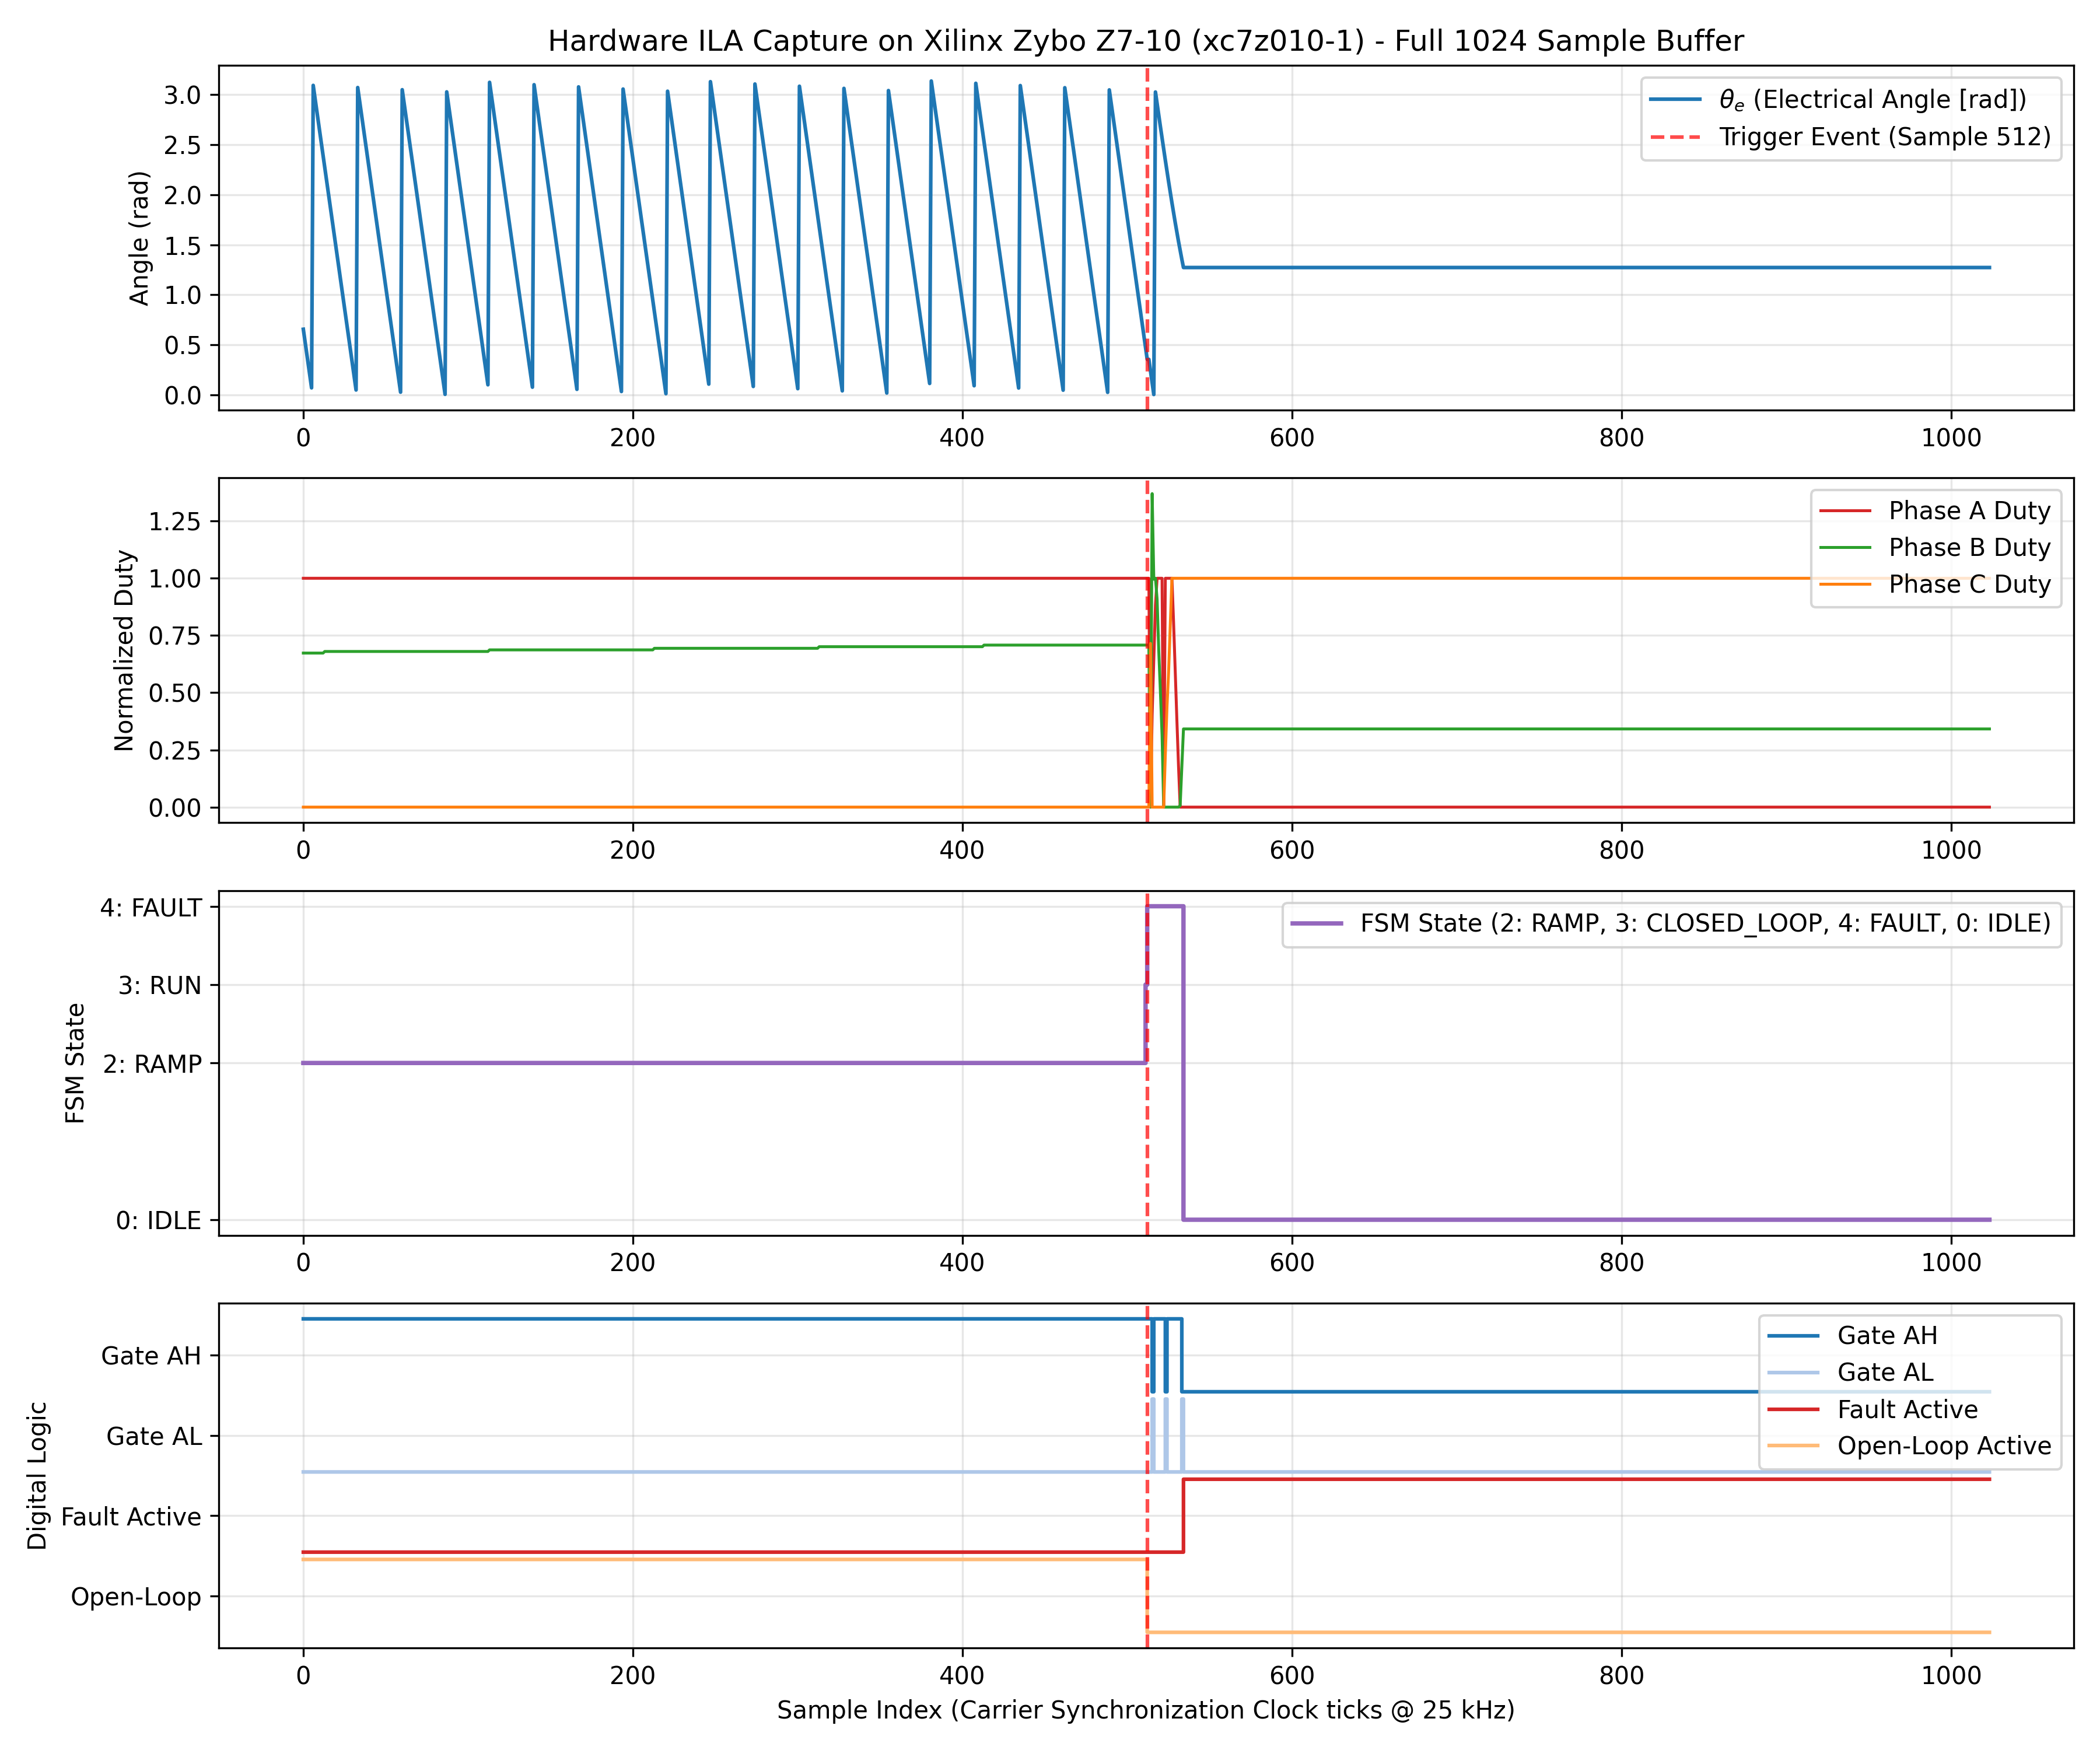
\includegraphics[width=\linewidth]{06_reports/figures/ila_hardware_capture.png}
  \caption{ILA capture of FOC startup and handover.}
  \label{fig:ila}
\end{minipage}\hfill
\begin{minipage}{0.48\linewidth}\centering
  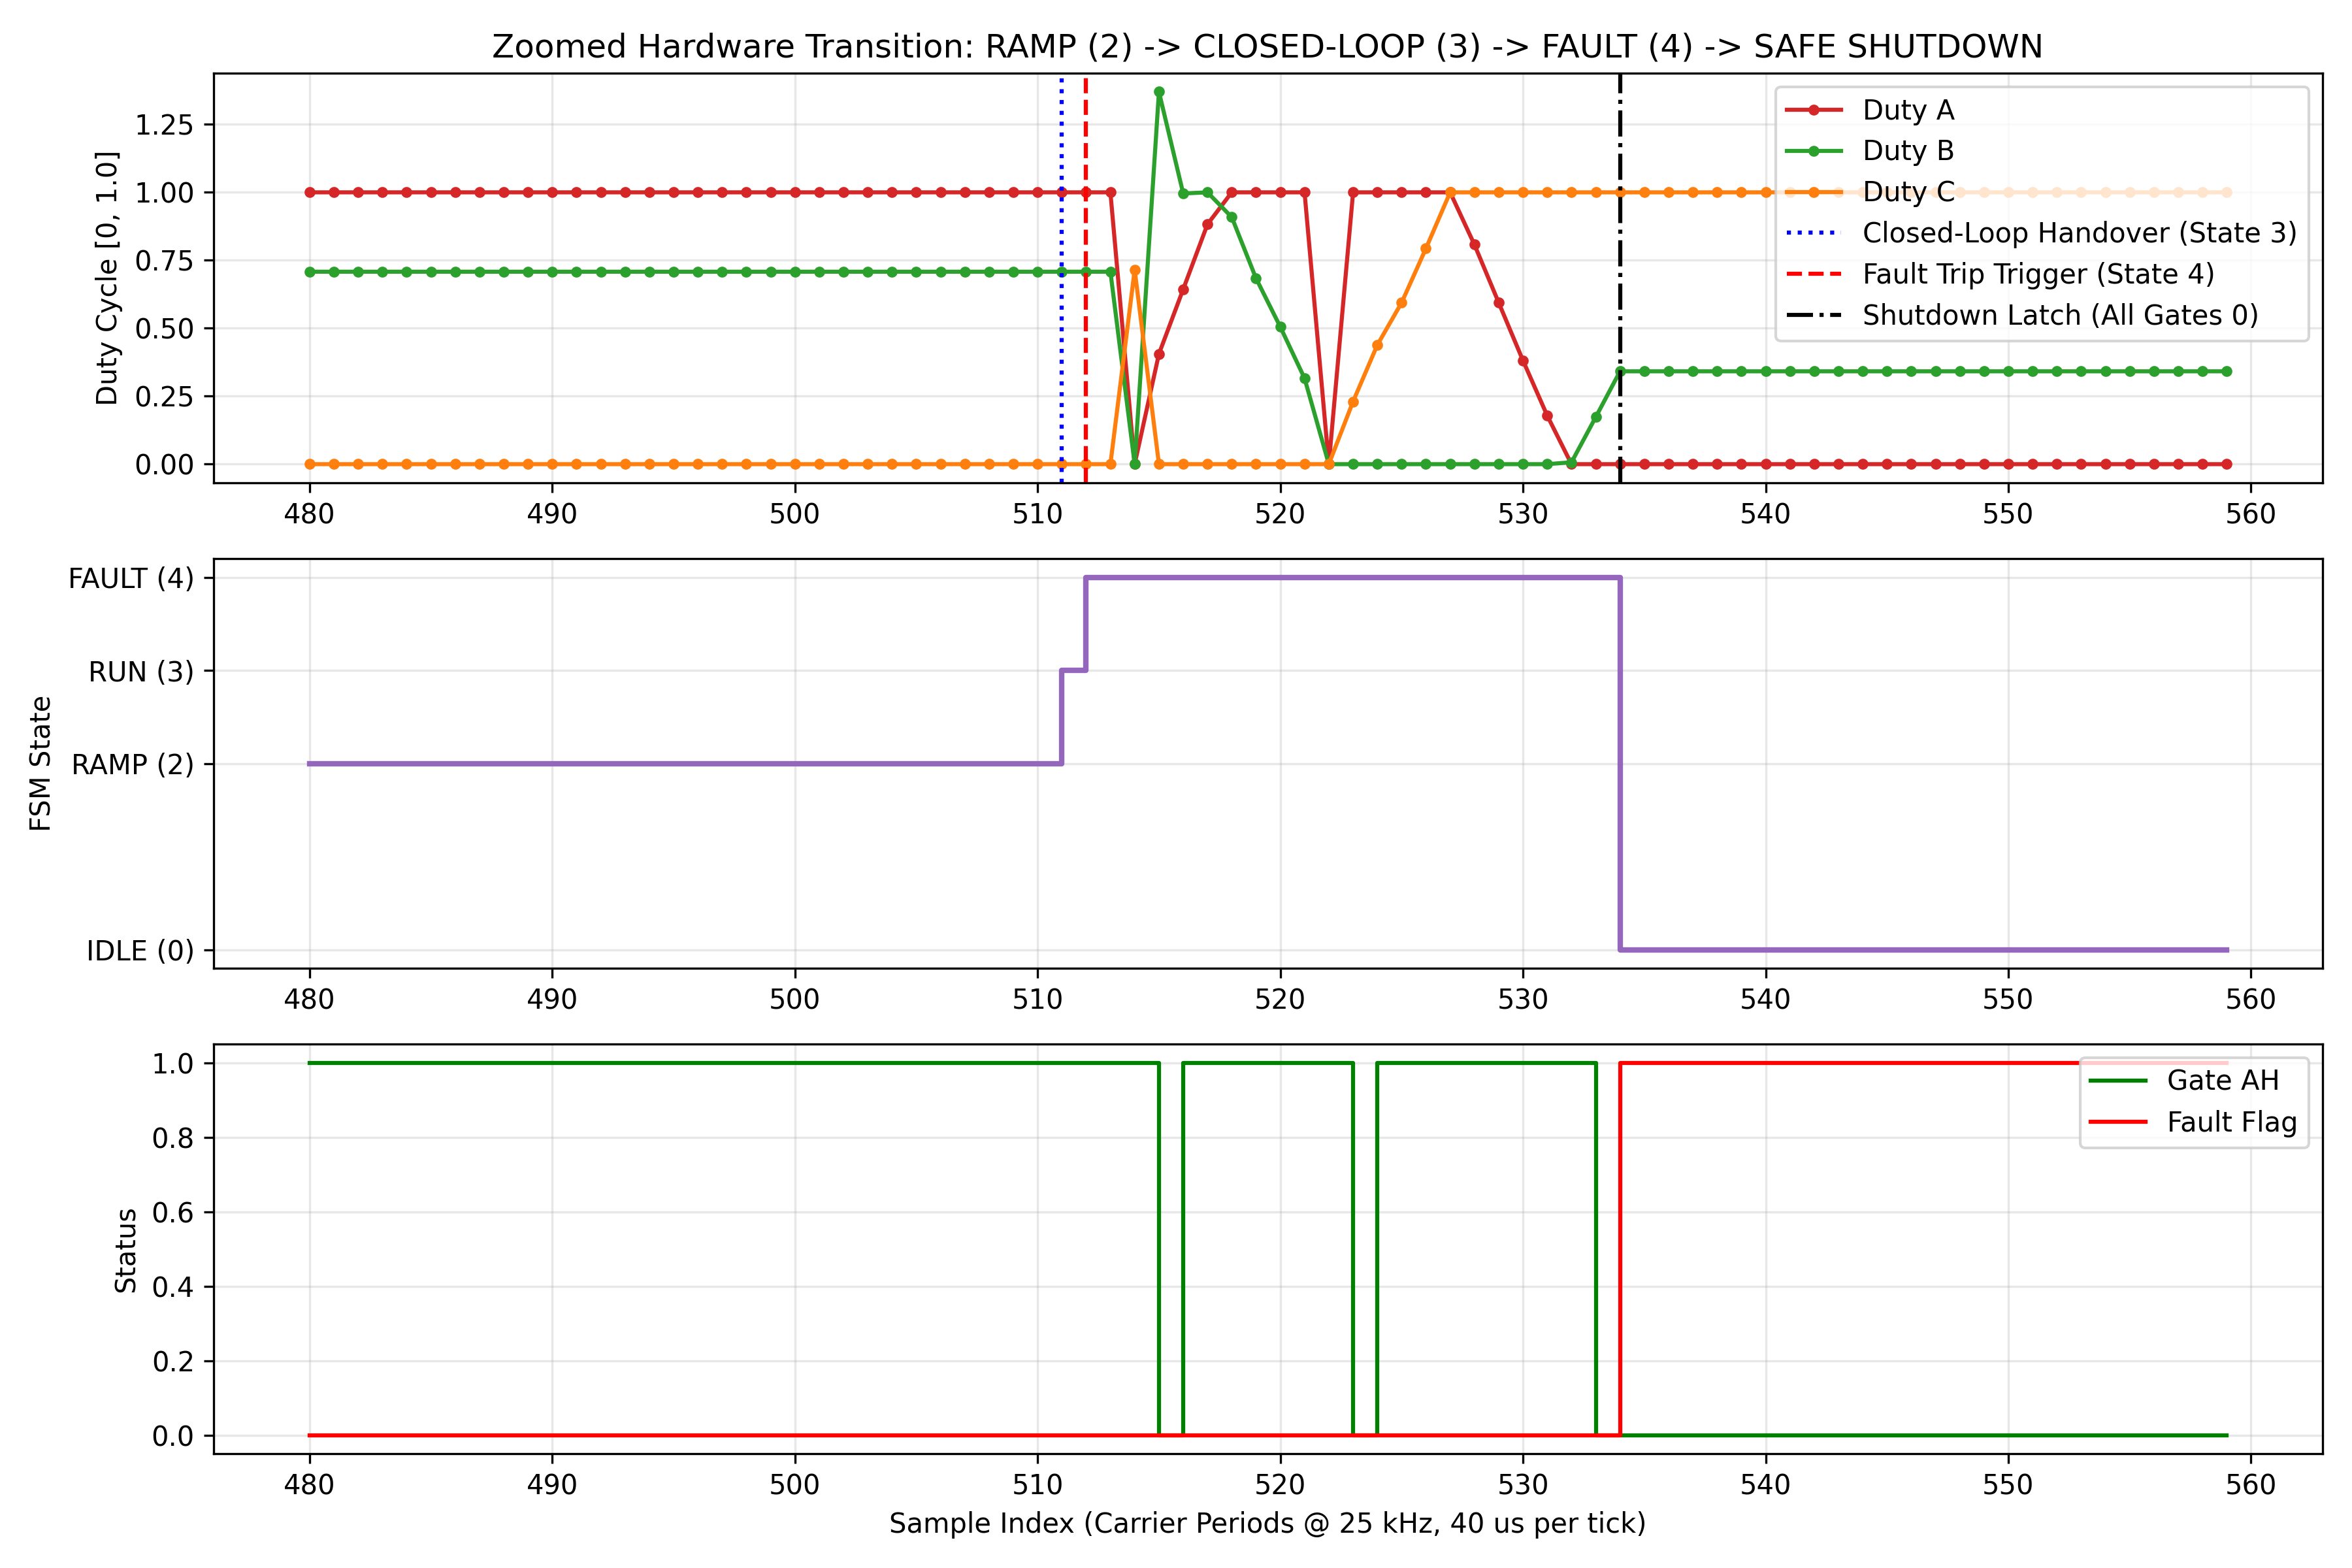
\includegraphics[width=\linewidth]{06_reports/figures/ila_transition_zoom.png}
  \caption{ILA zoom: dead-time shoot-through interlock.}
  \label{fig:ilaZoom}
\end{minipage}
\end{figure}

The hardware capture confirms:
\begin{itemize}
  \item Smooth transition through startup states (\texttt{ALIGN} $\to$ \texttt{RAMP} $\to$ \texttt{HANDOVER} $\to$ \texttt{RUNNING}).
  \item Mutual exclusion of complementary gates ($G_H \wedge G_L = 0$) across all 81 captured switching edges.
  \item Hardware dead-time gap $\ge 16$\,ns (2 cycles), preventing shoot-through.
  \item Instantaneous trip to safe mode within 1 clock cycle upon assertion of over-current fault.
\end{itemize}

%% =====================================================================
\section{Discussion and Limitations}
\label{sec:discussion}

\textbf{What Worked:}
\begin{enumerate}
  \item Timing closed at 125\,MHz on a slow -1 speed grade FPGA without requiring multicycle paths.
  \item The hand-HLS 2-DSP schedule matches the paper's intent and proved highly area-efficient.
  \item The CORDIC vector-rotator reproduced from Tufekci et al.~\cite{tufekci2020} cut inner-loop latency in half (51 cycles) while requiring only 1~DSP slice.
  \item NuSMV and SymbiYosys formally proved shoot-through immunity.
\end{enumerate}

\textbf{Limitations:}
\begin{enumerate}
  \item \textbf{Plant Voltage Saturation:} At 1000\,RPM, terminal voltage requirements exceed the 24\,V supply limit, causing field-weakening saturation.
  \item \textbf{Total DSP Count:} While the inner FOC loop uses only 1--2 DSPs, the total system footprint reaches 44 DSPs due to unconstrained SVPWM dwell-scaling (20 DSPs) and the on-chip HIL plant ODE solvers (14 DSPs).
  \item \textbf{Induction Depth:} RTL model checking was bounded at depth 20; unbounded proofs were verified via the abstracted NuSMV Kripke structure.
\end{enumerate}

%% =====================================================================
\section{Conclusion and Future Work}
\label{sec:conclusion}

We designed and verified an FPGA-based FOC motor controller with on-chip PMSM HIL plant on the Digilent Zybo Z7-10. Timing closed at 125\,MHz (WNS\,$=+0.321$\,ns). Hand HLS constrained the inner loop to 2~DSPs at 96~cycles. Reproducing the CORDIC-based architecture from Tufekci et al.~\cite{tufekci2020} achieved 1~DSP and 51~cycles latency (46.9\% reduction). Formal verification (8 CTL properties in NuSMV and BMC depth 20 in SymbiYosys) proved zero shoot-through, and 500/500 golden test vectors passed with $\le 1$\,LSB error. Future work includes implementing adaptive flux-weakening to mitigate high-speed voltage saturation and time-multiplexing the HIL plant to reduce overall chip DSP usage.

%% =====================================================================
\section*{Contribution Statement and Acknowledgements}
\addcontentsline{toc}{section}{Contribution Statement and Acknowledgements}
\label{sec:contrib}

\begin{table}[H]\centering\small
\begin{tabularx}{\linewidth}{@{}lX@{}}
\toprule
\textbf{Member} & \textbf{Main Contributions}\\
\midrule
\studentA & Research paper reproduction and comparative benchmarking (Tufekci et al.~\cite{tufekci2020} CORDIC-based FOC architecture in \texttt{cordic\_rotate.sv} and \texttt{foc\_current\_cordic.sv}), paper testbench verification (\texttt{tb\_paper\_cordic.sv}), simulation testbench execution, formal verification (NuSMV CTL model checking, SymbiYosys BMC), joint FPGA bring-up and ILA hardware validation, and report writing.\\
\studentB & Complete baseline FOC project design and architecture: Python fixed-point golden model, RTL datapath and plant (\texttt{clarke.sv}, \texttt{park.sv}, \texttt{inv\_park.sv}, \texttt{svpwm.sv},   \texttt{current\_pi.sv}, \texttt{dead\_time.sv}, \texttt{pmsm\_plant.sv}, \texttt{rv32i\_core.sv}, \texttt{apb\_csr.sv}), Hand HLS (CDFG dataflow, FDS/ILP 2-DSP schedule \texttt{foc\_shared\_2dsp.sv}), joint FPGA timing closure at 125\,MHz, ILA hardware demo, and report writing.\\
\bottomrule
\end{tabularx}
\end{table}

Both members actively collaborated on simulation-based verification, FPGA hardware testing, ILA logic analyzer debugging, and report authoring. Both authors reviewed all components and can defend every aspect of the design.

\textbf{Open-Source IP Used:} AMD/Xilinx Vivado 2025.1 ILA debug core (for in-system hardware logic probing). All motor control algorithms, coordinate transforms, filter logic, and processor peripherals are original code.

\textbf{AI-Tool Use:} Antigravity (Google DeepMind) AI assistant was utilised to review HLS scheduling tables, cross-check CTL syntax, and format LaTeX tables. All RTL, verification code, and analysis were written and validated by the authors.

%% =====================================================================
\begin{thebibliography}{99}
\bibitem{tufekci2020}
B.~Tufekci, B.~Onal, H.~Dere, and H.\,F.~Ugurdag, ``Efficient FPGA Implementation of Field Oriented Control for 3-Phase Machine Drives,'' in \emph{Proc.\ IEEE East-West Design \& Test Symposium (EWDTS)}, Varna, Bulgaria, 2020, pp.~1--5, doi: 10.1109/EWDTS50664.2020.9224884.

\bibitem{holmes2003}
D.\,G.~Holmes and T.\,A.~Lipo, \emph{Pulse Width Modulation for Power Converters: Principles and Practice}. IEEE Press / Wiley-Interscience, 2003.

\bibitem{monmasson2007}
E.~Monmasson and M.\,N.~Cirstea, ``FPGA Design Methodology for Industrial Control Systems---A Review,'' \emph{IEEE Trans.\ Ind.\ Electron.}, vol.~54, no.~4, pp.~1824--1842, Aug.~2007.

\bibitem{kung2007}
Y.-S.~Kung and G.-S.~Tsai, ``FPGA-Based Speed Control IC for PMSM Drive With Adaptive Fuzzy Control,'' \emph{IEEE Trans.\ Power Electron.}, vol.~22, no.~6, pp.~2476--2486, Nov.~2007.
\end{thebibliography}

%% =====================================================================
\appendix
\section{Repository and How to Reproduce}
\label{app:repo}

\begin{lstlisting}[language=bash,numbers=none]
# 1. Run complete Vivado synthesis, implementation, and bitstream generation
vivado -mode batch -source 08_scripts/run_project_implementation.tcl

# 2. Run top-level closed-loop system simulation (tb_foc_top)
vivado -mode batch -source 08_scripts/run_tb_foc_top.tcl

# 3. Run paper architecture stand-alone simulation and out-of-context synthesis
vivado -mode batch -source 05_paper_impl/vivado_synth_paper.tcl

# 4. Run NuSMV formal model checker
nusmv 04_formal/nusmv/shoot_through.smv

# 5. Run SymbiYosys bounded model checker
cd 04_formal/sby && sby -f shoot_through.sby

# 6. Regenerate Python golden model test vectors
cd 02_golden_model && python foc_golden.py && python generate_pipeline_vectors.py
\end{lstlisting}

\section{NuSMV Model (excerpt)}
\label{app:nusmv}
The half-bridge dead-time protection controller and shoot-through safety invariant are modelled in NuSMV (\texttt{04\_formal/nusmv/shoot\_through.smv}) as listed below:

\begin{lstlisting}[language=SMV,caption={NuSMV shoot-through invariant model (excerpt).},label={lst:nusmv}]
MODULE main
VAR
  clk    : boolean;
  rst    : boolean;
  fault  : boolean;
  pwm_in : boolean;
  state  : {ST_OFF, ST_HIGH, ST_LOW};
  timer  : 0..3;
  gate_h : boolean;
  gate_l : boolean;

ASSIGN
  init(state)  := ST_OFF;
  init(timer)  := 0;
  init(gate_h) := FALSE;
  init(gate_l) := FALSE;

  next(state) :=
    case
      rst | fault : ST_OFF;
      state = ST_OFF & pwm_in  : ST_HIGH;
      state = ST_OFF & !pwm_in : ST_LOW;
      state = ST_HIGH & !pwm_in: ST_OFF;
      state = ST_LOW  & pwm_in : ST_OFF;
      TRUE : state;
    esac;

  next(timer) :=
    case
      rst | fault : 0;
      state != next(state) & next(state) = ST_OFF : 2; -- 2 cycles dead time
      timer > 0 : timer - 1;
      TRUE : 0;
    esac;

  next(gate_h) :=
    case
      rst | fault : FALSE;
      next(state) = ST_HIGH & next(timer) = 0 : TRUE;
      TRUE : FALSE;
    esac;

  next(gate_l) :=
    case
      rst | fault : FALSE;
      next(state) = ST_LOW & next(timer) = 0 : TRUE;
      TRUE : FALSE;
    esac;

-- Invariants verified:
CTLSPEC AG !(gate_h & gate_l)
CTLSPEC AG ((rst | fault) -> (!gate_h & !gate_l))
CTLSPEC AG (timer > 0 -> (!gate_h & !gate_l))
CTLSPEC AG ((state = ST_OFF & pwm_in & !fault) -> AF gate_h)
CTLSPEC AG ((state = ST_OFF & !pwm_in & !fault) -> AF gate_l)
CTLSPEC AG EF (state = ST_OFF)
CTLSPEC AG (fault -> AX (state = ST_OFF))
CTLSPEC AG (EX TRUE)
\end{lstlisting}

\end{document}
